\documentclass[11pt]{article}

\bibliographystyle{abbrv}

\usepackage{amsfonts}

\usepackage{amsthm}

\usepackage{amssymb}

\usepackage{amsmath}

\usepackage{enumerate}

\usepackage{fancyhdr}

\usepackage{mathabx}

\usepackage{verbatim}

\usepackage{tikz}

%%%%%%%%%%%%%%%%%%%%%%%%%%%%%%%%%%%%%%%%%%%%%%%%%%%%%%%
%% Setting for the nice arrows and nodes graphs  %%%%%%
%%%%%%%%%%%%%%%%%%%%%%%%%%%%%%%%%%%%%%%%%%%%%%%%%%%%%%%

\usetikzlibrary{arrows,positioning,decorations.markings} 
\tikzset{
    %Define standard arrow tip
    >=stealth',
    %Define style for boxes
    punkt/.style={
           rectangle,
           rounded corners,
           draw=black, very thick,
           text width=6.5em,
           minimum height=2em,
           text centered},
    % Define arrow style
    pil/.style={
           ->,
           thick,
           shorten <=2pt,
           shorten >=2pt,}
}
\tikzstyle{vecArrow} = [thick, decoration={markings,mark=at position
   1 with {\arrow[semithick]{open triangle 60}}},
   double distance=1.4pt, shorten >= 5.5pt,
   preaction = {decorate},
   postaction = {draw,line width=1.4pt, white,shorten >= 4.5pt}]
\tikzstyle{innerWhite} = [semithick, white,line width=1.4pt, shorten >= 4.5pt]

%%%%%%%%%%%%%%%%%%%%%%%%%%%%%%%%%%%%%%%%%%%%%%%%%%%%%%%%
%%%%%%%%%%%%%%%%%%%%%%%%%%%%%%%%%%%%%%%%%%%%%%%%%%%%%%%%

\usepackage[all]{xy}

% \usepackage{showlabels}
%  Formatting matters
% original dimensions

\textwidth=5.75truein
\textheight=8.5truein


% dimensions to play with
%\textheight=8.0truein   %for mac
%\textwidth=6.0truein

\oddsidemargin=0.3truein
\evensidemargin=0.3truein

%\topmargin=-0.35truein %original
\topmargin=-0.25truein
% \headheight=0.16truein
\headheight=13pt
\headsep=0.3truein

\footskip=0.5truein

\parindent=18pt
\tolerance=6000
\parskip=0pt



\linespread{1.02}


\newcommand{\N}{\mathbb{N}}

\newcommand{\Z}{\mathbb{Z}}

\newcommand{\R}{\mathbb{R}}

\newcommand{\Q}{\mathbb{Q}}

\newcommand{\C}{\mathbb{C}}

\newcommand{\T}{\mathbb{T}}

\newcommand{\h}{\mathcal{H}}

\newcommand{\Manoa}{M\=anoa}

\newcommand{\Hawaii}{Hawai\kern.05em`\kern.05em\relax i}

\theoremstyle{plain}
\newtheorem{theorem}{Theorem}[section]
\newtheorem{lemma}[theorem]{Lemma}
\newtheorem{corollary}[theorem]{Corollary}
\newtheorem{proposition}[theorem]{Proposition}
\newtheorem{conjecture}[theorem]{Conjecture}
\newtheorem{definition-theorem}[theorem]{Definition / Theorem}
\newtheorem{project}[theorem]{Project}

% without a number

\newtheorem*{conjecture*}{Conjecture}
\newtheorem*{theorem*}{Theorem}

\theoremstyle{definition}
\newtheorem{definition}[theorem]{Definition}
\newtheorem{example}[theorem]{Example}
\newtheorem{notation}[theorem]{Notation}
\newtheorem{convention}[theorem]{Convention}


\theoremstyle{remark}
\newtheorem{remark}[theorem]{Remark}
\newtheorem{remarks}[theorem]{Remarks}

% without a number

\newtheorem*{example*}{Example}  
\newtheorem*{remark*}{Remark}

\begin{document}

\section*{Project Description}

%Cl\'{e}ment Dell'Aiera and Rufus Willett - $K$-theory, groups, and groupoids.\\


In the first section below we discuss results (both intellectual merit and broader impacts) from prior support, in the second section we discuss the intellectual merit of the proposed project, and in the third section we discuss its broader impacts.
 
\section{Results from prior NSF Support}

PI Dell'Aiera has no prior support from the US NSF.  

%%%%%%%%%%%%%%%%%%%%%%%%%%%%
%%%%%%%%%%%%%%%%%%%%%%%%%%%%
\section{Current proposal}
This section describes several research projects that we submit for the proposal for the next three years. We organized these into two sections entitled \textit{Weak decompositions} and \textit{Quantum groups}. Before this, we first give some background. The author will try to explain how the current questions in \textit{Operator Algebras} and \textit{Noncommutative Geometry} they are interested in are related to other parts of mathematics. Our point of view is to see our activity as an offspring of Grothendieck's work on tensor products of Banach spaces.    

\subsection{From approximation properties to the K\"unneth formula in operator $K$-theory and the Universal Coefficient Theorem}

An important part of Operator Algebras as a field can be described as attempting to answer questions arising in Functional Analysis using other seemingly unrelated fields, the most common being Topological Dynamics, Group and Geometric Group theory. A good starting point to understand these preocupations is the work of Alexander Grothendieck on tensor products of topological vector spaces. \\

At the time, starting his PhD in Nancy, Grothendieck was asked by Laurent Schwartz to develop a theory of tensor products for topological vector spaces. This question was motivated by the kernel theorem, whose proof was found to be too involved by Laurent Schwartz in the general case, whereas the finite dimensional case reduces to the fact that 
\[V^*\otimes W \cong Hom(V,W),\] 
where $V$ and $W$ are finite dimensional vector spaces and $Hom(V,W)$ is the space of linear maps $V\rightarrow W$. Having topological tensor products in one's toolbox led to hope for a simpler and more natural proof. The rest of the story is well known: Grothendieck found that one could define a lot of completions of the algebraic tensor products. Spaces admitting only one such completion were called \textit{nucl\'eaires}, or nuclear, after the kernel theorem (\textit{nucl\'eaires} means ``related to the kernel" in French).\\

The paper \textit{R\'esum\'e de la th\'eorie m\'etrique des produits tensoriels topologiques} \cite{GrothendieckResume}, commonly know as the Resum\'e, enhanced a vast research program. It specialized the work to the case of Banach spaces. Surprisingly, the paper did not attract a lot of attention at the time of its publication, maybe because the trend was back then to focus on locally convex spaces. The paper was rediscovered fifteen years later. See Pisier's paper \cite{PisierSurvey} for a very nice survey on the subject.\\

Approximation theory for $C^*$-algebras is a direct offspring of this work. The idea is to study properties of various constructions such as tensor products or crossed-products (which is a twisted version of tensor products) of $C^*$-algebras. It is very useful in that case to use spaces of functions on a topological group as a tool to construct exotic examples. Let me illustrate this by the following example.\\

John Von Neumann defined a property on groups called \textit{amenability} as follows. A discrete countable group $\Gamma$ is said to be amenable if there exists an invariant mean (i.e. $\Gamma$-invariant linear positive functional) $m: l^\infty(\Gamma)\rightarrow \C$. Now, the group ring $\C[\Gamma]$ is a $*$-algebra w.r.t. the convolution as a product and $(z. \gamma)^* = \overline{z}\gamma^{-1}$. This algebra can be represented as a self adjoint subalgebra of the bounded operators on the complex Hilbert space $l^2\Gamma$ by what is called the left regular representation $\lambda_\Gamma: \C[\Gamma]\rightarrow B(l^2\Gamma)$. The reduced $C^*$-algebra of the group $\Gamma$ is defined as the closure of the image of the regular representation.\\

It turns out that, for such a group $\Gamma$, this $C^*$-algebra is nuclear iff $\Gamma$ is amenable. Thus, examples of nonamenable groups (like any nonabelian free group) provide instances of nonnuclear $C^*$-algebras. This example is typical of how a completely group theoretic property can be used to provide contructions of Banach algebras with interesting properties. Many other areas of mathematics contribute to fuel new ideas in operator algebras. A nice object which is general enough to encompass all of these constructions and provides easily a $C^*$-algebra is a \textit{groupoid}. For our purpose, the reader only needs to know that a groupoid is meant to be two locally compact spaces: the objects $G^0$ and the arrows $G$. $G$ is ``group like" in the sense that it has a partial multiplication law and every arrow has an inverse for it. The difference with a group is that $G$ sits over the base space $G^0$: every arrow has a source and a target in $G^0$.\\  

This extra flexibility makes groupoids very versatile. Indeed, out of an action by homeomorphisms of a group $\Gamma$ on a topological space $\Omega$ or out of a metric space $X$, one can build groupoids (respectively the action groupoid $\Omega \rtimes \Gamma$ and the coarse groupoid $G(X)$ \cite{SkTuYu}) nice enough to have convolution algebras. \\  
%Amenability was of uttermost importance in the classification of factors obtained by Connes \cite{}. \\ 

% Examples from http://www.texample.net/tikz/examples/borrowers-and-lenders/ 
% and http://www.texample.net/tikz/examples/double-arrows/

%%%%%%%%%%%%%%%%%%%%%%%%%%%%%%%%%%%%%%%%%%%%%%%%%%%%%%%%%%%%%%%%%%%%%%%%%%%
\[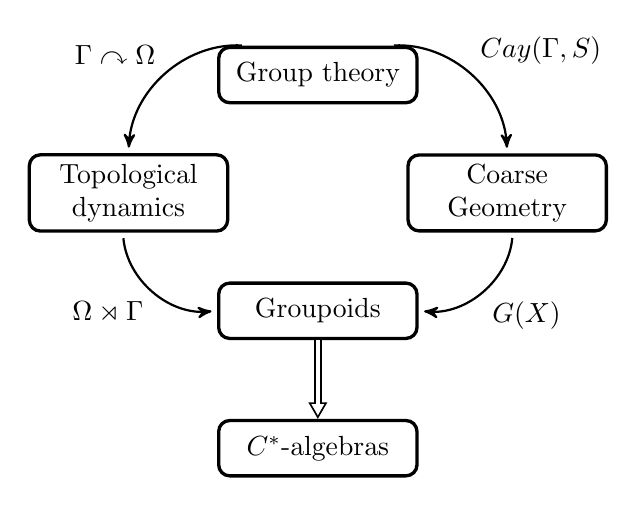
\begin{tikzpicture}[node distance=1cm, auto,]
 %nodes
\node[punkt] (C) {$C^*$-algebras};\\
\node[punkt, above=of C] (G) {Groupoids};
\node[above=of G] (dummy) {};
\node[punkt, right=of dummy] (CG) {Coarse Geometry}
	edge[pil, bend left=45] node[auto] {$G(X)$} (G.east); 
\node[punkt, left=of dummy] (TD) {Topological dynamics}
	edge[pil, bend right=45] node[auto] [below left] {$\Omega\rtimes \Gamma$} (G.west); 
\node[punkt, above=of dummy] (GT) {Group theory}
	edge[pil, bend left=45] node[auto] {$Cay(\Gamma,S)$} (CG.north) 
	edge[pil, bend right=45] node[auto] [above left] {$\Gamma \curvearrowright \Omega$} (TD.north);

\draw[vecArrow] (G) to (C);
\end{tikzpicture}\]
%%%%%%%%%%%%%%%%%%%%%%%%%%%%%%%%%%%%%%%%%%%%%%%%%%%%%%%%%%%%%%%%%%%%%%%%%%%

Taking a property in any of these areas, trying to define it in the setting of groupoids, then unravelling the definition in another setting has proven to be a very fruitful strategy. For instance, amenability can be easily defined for locally compact groupoids \cite{anantharaman2000amenable}. But if one looks at the coarse groupoid $G(X)$ of a metric space, saying it is amenable is equivalent to say that $X$ has Yu's property (A) (a \textit{coarse} version of amenability). Another direction is to use properties of groupoids to build interesting classes of $C^*$-algebras. For instance, second countable locally compact amenable groupoids have reduced $C^*$-algebras that are known to satisfy the K\"unneth formula. \\

Over the years, other properties have been found to be of interest. Without pretending to be exhaustive, let us just mention exactness, simplicity, finite nuclear dimension, the UCT class, the Bootstrap class,... Usually these classes are important because of their relation to Elliot's classification program, or to topology and geometry. \\

One of the objects of importance for $C^*$-algebras are the \textit{operator $K$-theory groups} $K_0(A)$ and $K_1(A)$, which are homotopy invariant abelian groups associated to any $C^*$-algebras. Let us just say that $K_0(A)$ is built out of equivalence classes of projections in $M_n(A)$, while $K_1(A)$ is built from equivalence classes of unitaries in $M_n(A)$. These groups are a generalized cohomology theory on the category of $C^*$-algebras. Georges Elliott suggested that all separable nuclear $C^*$-algebras should be classifiable by ``$K$-theoretic'' invariants. While seen as unreachable at the time of its statement, Elliott's conjecture cristallised last year as the following theorem (see W. Winter's survey \cite{WinterClassification}).

\begin{theorem}\label{classification}(By many, many hands \cite{WinterClassification}) All separable simple unital UCT $C^*$-algebras of finite nuclear dimension are classifiable.
\end{theorem}

This result, together with the fact that the $K$-groups are notoriously difficult to compute, give motivations to the following problems:
\begin{enumerate}
\item define special families of $C^*$-algebras and prove that they satisfy the conditions of the classification theorem \ref{classification},
\item enlarge the range of applicability of theorem \ref{classification},
\item find a way to compute the $K$-theory groups.
\end{enumerate}    

The first two points are very active branches of research right now, and much work has been devoted to find a way to prove that finite nuclear dimension for $C^*$-algebras implies the UCT. UCT stands for Universal Coefficients Theorem, and a $C^*$-algebra is said to belong to the UCT class if the Kasparov abelian groups $KK_0(A,B)$ and $KK_1(A,B)$ can be computed for every $C^*$-algebras $B$ from the $K$-theory groups of $A$ and $B$. A very similar class is that of $C^*$-algebras that satisfy the K\"unneth formula. The map $\alpha: [p]\otimes [q] \mapsto [p\otimes q]$ induces a product in $K$-theory (at the level of $K_0$, then similar formulas do the jobs for $K_*$). A $C^*$-algebra $A$ is said to satisfy the K\"unneth formula if 

\[\alpha: K_*(A) \otimes K_*(B)\rightarrow K_*(A\otimes B)\]
 is an isomorphism for every $C^*$-algebra $B$ such that $K_*(B)$ is free abelian. It is know to be true for every $C^*$-algebra in the \textit{Bootstrap class}, i.e. that is $KK$-equivalent to a commutative $C^*$-algebra ($KK$-equivalence is a suitable notion of weak equivalence for $C^*$-algebras).\\

On the other hand, the $K$-groups are computable for $C^*$-algebras coming from groups satisfying the Baum-Connes conjecture. In \cite{BaumConnesHigson}, P. Baum, A. Connes and N. Higson suggested that a certain group homomorphism
\[\mu_G : K_*^{top}(\underline E G) \rightarrow K_*(C_r^*(G)), \]
called the assembly map, is an isomorphism. Here, 
\begin{itemize}
\item[$\bullet$] $\underline E G$ is the classifying space for proper actions of $G$, a CW-complex associated to $G$,
\item[$\bullet$] $K_*^{top}(X)$ is, for every left $G$-space $X$, the \textit{$G$-equivariant analytic $K$-homology} of $X$, a classical homology group that can be computed by the traditional means of algebraic topology,
\item[$\bullet$] and of course $K_*(C_r^*(G))$ stands for the $K$-theory groups of the reduced $C^*$-algebra of $G$. 
\end{itemize}

This conjecture is a far reaching generalization of the Atiyah-Singer index theorem, and is know to be true for every group which has the Haagerup property (Gromov's a-T-menability). In particular, every amenable group satisfies the Baum-Connes conjecture. The conjecture has a version with coefficients and can also be generalized to the setting of groupoids. The conjecture with coefficients is known to be false for groups, but no counterexample is known at this moment for the original statement. The case of groupoids in strikingly different: in \cite{SkTuYu}, Skandalis, Tu and Yu build very simple examples of groupoids which do not satisfy the Baum-Connes conjecture (already without coefficients).\\

Another reason why computation of $K$-theory groups and the Baum-Connes conjecture is so interesting is its link with classical geometry and topology. Indeed, if $G=\pi_1(M)$ is the fundamental group of a closed aspherical manifold, the assembly map $\mu_G$ specializes to 
\[\mu_G : K_*(M)\rightarrow K_*(C^*_r(G)).\]
The injectivity of $\mu_G$ proves the Novikov conjecture for $M$, which states the homotopy invariance of higher signatures of $M$. More precisely:

\begin{conjecture} Let $M$ be a smooth oriented closed manifold, 
$[M]\in H_{dim(M)}(M,\mathbb Q)$ its fundamental class and
$ L(M)\in H^{*}(M,\mathbb Q)$ its $L$-class. Let $\Gamma$ a discrete group and $B\Gamma$ its classifying space. 
For any map $f: M \rightarrow B\Gamma$, define the higher signature 
\[\sigma_x(M,f) = \langle L(M)\cup f^*(x),[M] \rangle \quad \forall x \in H(B\Gamma, \mathbb Q).\]
The Novikov conjecture states that for every orientation preserving homotopy equivalence $\phi : N\rightarrow M$,
\[\sigma_x(M,f)= \sigma_x(N,f\circ \phi).\]
\end{conjecture}

Injectivity of the assembly map has other important consequences. If $M$ is supposed to be a spin manifold, then it implies that $M$ does not admit a metric of positive scalar curvature (Gromov-Lawson-Rosenberg conjecture). Surjectivity of $\mu_G$ implies that $C^*_r(G)$ does not contain any non trivial idempotents.\\

We will present several projects that are related to these questions. 
\begin{enumerate}
\item In recent work \cite{DelBo18}, the author and Chrisitan B\"onicke have proven that the K\"unneth formula holds for Roe algebras of metric spaces that admit a coarse embedding into Hilbert space. This is done by using topological groupoid techniques combined with using the Baum-Connes assembly map. The core of the proof relies on stability of the K\"unneth formula with respect to a weak type of decomposition of \'etale groupoids, inspired by notions such as asymptotic dimension and finite decomposition complexity in geometric group theory and coarse geometry. \\

\textbf{Question:} Is the Baum-Connes conjecture also stable by this kind of decomposition ?\\

This seems plausible by recent results of H. Oyono-Oyono and G. Yu \cite{OY3}, where they proved the coarse Baum-Connes conjecture for groups with finite decomposition complexity. An interesting point is the existence of groupoids that decompose w.r.t. a family of a-T-menable groupoids but are not themselves a-T-menable. If the question can be answered positively, this would provide new examples of groupoids that satisfiy the Baum-Connes conjecture.     

\item The use of \textit{weak decomposition} of groupoids (or of coarse spaces) uses intensively \textit{controlled $K$-theory}, which is a refinement of operator $K$-theory that was developed by Oyono-Oyono and Yu \cite{OY2}. Controlled $K$-theory is defined as a family of groups indexed by two numbers, which when one takes to $0$ and $\infty$ recovers $K$-theory. In the author's thesis, controlled $K$-theory was slightly generalized in order to be applicable to groupoid $C^*$-algebras and quantum groups. The case of quantum groups was surprising and not expected, and asks for a development of these techniques to that setting. We will present several projects that could be understood as an attempt to use \textit{coarse geometric techniques} for quantum groups.  
\end{enumerate}

The rest of the piece will be to give details and context to these ideas.

\subsection{Weak decompositions}

Recall that a metric space $X$ has \textit{asymptotic dimension} less than $d$ if, for every $r>0$, there exists a decomposition of $X$
\[X = X_0 \cup X_1 \cup ... \cup X_d,\]
into $d+1$ subspaces that are $r$-disjoint family of uniformly bounded subsets, i.e. \[X_i = \coprod_r X_{i,j}\] with $\sup_{i,j} diam(X_{i,j})<\infty$. Here, $\coprod_r$ means $r$-disjoint union, i.e. $d(X_{ij},X_{ik})>r$ for $j\neq k$. A nice example to keep in mind is $\Z$, which is of asymptotic dimension $1$. The upper bound can be seen by looking at the decomposition 
\[ \Z = \coprod_k [ \ 20rk, 20rk+10r \ ] \cup \coprod_k [ \  (2k+1)10r , (2k+1)10r+10r \ ] \] It is a fact that $\Z^n$ has asymptotic dimension $n$. \\

If one looks at $\Gamma=\bigoplus_{n\in \N} \Z$ with the left invariant metric 
\[ l(a)= \sum_n n|a_n|, \quad \forall a = (a_n)_{n \geq 0}\] it is easily seen as being of infinite asymptotic dimension. Yet, it still admits a similar decomposition, if one is allowed to decompose in two steps. Indeed, $\Gamma$ identifies with the collection of finitely supported functions $\N \rightarrow \Z$. Define $\Gamma_i^{(1)}$ to be the space of such functions supported on $\coprod_k [| \ (2k+i)r, (2k+i)r+r \ |]$ for $i=0,1$. Each of the two pieces is an $r$-disjoint union of spaces almost isometric to $\Z^r$, which by finite asymptotic dimension can also be decomposed in the same way, only this time by a uniformly bounded family.\\ 

The relevant property for our purpose is the decomposition of a space, for every $r$, into $r$-disjoint families. If one has such a decomposition
\[X = X_0 \cup X_1 , \quad X_i = \coprod_r X_{ij} \ .\]
%one can look at the $C^*$-algebras
%\[C^*(X)\] 

When $X$ is a discrete countable group endowed with a left invariant metric, the coarse Baum-Connes conjecture for $X$ is know to imply the homotopy invariance of higher signatures for $\Gamma$ (Novikov conjecture). The $K$-theory of interest is that of the \textit{Roe algebra} $C^*(X)$. It is built as follows: let $H$ be the separable Hilbert space. $C^*(X)$ is the completion for the operator norm of the $*$-algebra of operators $a =(a_{xy})_{xy}\in B(l^2(X)\otimes H)$ which are:
\begin{itemize}
\item[$\bullet$] locally compact, i.e. $a_{xy}$ is a compact operator on $H$,
\item[$\bullet$] and of finite propagation, i.e. $\exists r> 0, \text{s.t. if } d(x,y)> r$ then $a_{xy}=0$.
\end{itemize}

In his celebrated work \cite{Yu1}, G. Yu proved the Novikov conjecture for spaces with finite asymptotic dimension using these kind of decompositions. Building on the techniques used in that article, H. Oyono-Oyono and G. Yu developed a refinment of $K$-theory called \textit{quantitative $K$-theory} which allows one to compute the $K$-theory of, for instance, the $C^*$-algebra $C^*(|\Gamma|) \cong l^\infty(\Gamma)\rtimes \Gamma$ from the $K$-theory of the subalgebras 
\[A_i = \prod_{j} C^*(X_{ij}),\]
which are actually products of compact operators. These are not closed ideals in $C^*(X)$, but are close enough of being so that a Mayer-Vietoris type sequence exists in \textit{quantitative $K$-theory}. this allows one to carry out the same type of proofs as in \cite{Yu1} and actually led to a proof of the coarse Baum-Connes conjecture for spaces with \textit{finite decomposition complexity}, hence of the Novikov conjecture for groups like $\bigoplus \Z$.  \\

The idea behind quantitative $K$-theory is to relax some relations in the definition of the $K$-groups. Recall that these are defined as equivalence classes of projections and unitaries in $C^*$-algebras. But being in a normed algebra offers some advantage compared to the algebraic setting: one can do approximation. The only additional ingredients one needs is a \textit{filtration} on the $C^*$-algebra, meaning a family of operator spaces $\{A_r\}_{r>0}$ such that $\cup_r A_r$ is dense in $A$ and $A_r A_s \subseteq A_{r+s}$. Then the quantitative $K$-group $K_0^{\varepsilon,r}(A)$ will be defined as equivalence classes of almost projections 
\[p=p^*\in M_n(A_r) \text{ s.t. } ||p^2 - p || <\varepsilon  \] 	 
and $K_1^{\varepsilon,r}(A)$ as equivalence classes of almost unitaries
\[u\in M_n(A_r) \text{ s.t. } ||uu^* - 1_n || <\varepsilon  \text{ and }  ||u^*u - 1_n || <\varepsilon \]

%\textbf{Filtered algebras}\\
The use of this kind of decomposition is not limited to prove the coarse Baum-Connes conjecture. In \cite{OY4}, Oyono-Oyono and Yu give a stability result for the K\"unneth formula that can be loosely summarized as: if a filtered $C^*$-algebra admits at every order $r$-approximate ideals such that these sub-$C^*$-algebras and their intersection satisfy a quantitative version of the K\"unneth formula, then the original algebra also does.\\
  
The author defined in his thesis (\cite{DellAieraThesis} and \cite{dell2018controlled}) a slight generalization of quantitative $K$-theory where the index $r$ can be any element of a \textit{coarse structure}, which is an abelian partially ordered semigroup equipped with a maximum. In the case of a groupoid $G$, the set of symmetric compact subsets of $G$ form a coarse structure $\mathcal E_G$ w.r.t. the inclusion and the composition
\[E \circ F = EF \cup FE,\]
where $EF = \{ xy \in G \text{ s.t. } x\in E, y\in F \ x\text{ and } y \text{ composable} \}$. Then the reduced and maximal $C^*$-algebras $C^*_r(G)$ and $C^*_{max}(G)$ are filtered by $\mathcal E_G$. The other case of interest, described in the next section, is the one of quantum groups.\\

This filtration makes it possible to use quantitative $K$-theory for any crossed-product of a $C^*$-algebra by an action of groupoid. Of course, there is a way to go from quantitative $K$-theory to actual $K$-theory (essentially by forgetting the filtration). The technical advantage of using the quantitative version resides in the existence of more exact sequences. More precisely, while in $K$-theory one needs a decomposition $A= I_0+I_1$ into ideals to use Mayer-Vietoris sequences, quantitative $K$-theory only requires ``approximate ideals'', which we don't want to define here. The point is that they exist even in simple $C^*$-algebras. \\

Building on previous work of Guentner, Oyono-Oyono, Willett and Yu (\cite{OY4}, \cite{GWY},\cite{GWY2}), the author and Christian B\"onicke define in \cite{DelBo18} the \textit{coarsely generated family} of a (countable) family of subgroupoids of a groupoid. One of the results of \cite{DelBo18} is the following.

\begin{theorem} Let $G$ be an \'etale groupoid and let $\mathcal G$ be such a family such that the reduced $C^*$-algebras of all the groupoids in $\mathcal C$ satisfy uniformly the quantitative K\"unneth formula. If $G$ belongs to the coarsely generated family of $\mathcal C$, then $C^*(G)$ satisfies the K\"unneth formula.         
\end{theorem}

This result can be thought as ``the K\"unneth formula for groupoids is stable with respect to finite decomposition". The natural question is to know if that can be done for the UCT class, and for the Baum-Connes conjecture.

\begin{project} Are the Baum-Connes conjecture and the UCT class stable with respect to finite decomposition?
\end{project}

In \cite{OY4}, Oyono-Oyono and Yu give a proof of the Novikov conjecture for FDC groups. This result suggests strongly that the Baum-Connes conjecture is stable w.r.t. finite decomposition at least for the restricted class of coarse groupoids. A good intuition is that whatever works for coarse groupoids usually extends to ample groupoids (which are \'etale groupoids with totally disconnected base space). \\

If true, this result would give new examples of groupoids which satisfy the Baum-Connes conjecture. Indeed, in \cite{DelBo18} we show that some groupoids finitely decompose over subgroupoids which are a-T-menable without being themselves a-T-menable (we can come up with an actual example). The biggest class of groupoids known to satisfy the Baum-Connes conjecture being the a-T-menable ones, one would then prove the Baum-Connes conjecture for a class strictly bigger.

%%%%%%%%%%%%%%%%%%%%%%%%%%%%
\subsection{Quantum groups}
%%%%%%%%%%%%%%%%%%%%%%%%%%%%

Quantum groups can be thought as \textit{noncommutative locally compact groups} in the same way that $C^*$-algebras can be seen as noncommutative spaces. This means that when the $C^*$-algebra is unital and commutative, it is isomorphic to the algebra of complex continuous functions on a compact group. In general, a compact quantum group will be given by a unital $C^*$-algebra $A$ together with a comultiplication $\Delta : A \rightarrow A \otimes A$ which satisfies technical properties. The basic examples of compact quantum groups are:
\begin{itemize}
\item[$\bullet$] $C(G)$ for $G$ a compact group, with comultiplication $\Delta(f)(x,y)= f(xy)$ (here $C(G)\otimes C(G)$ is identified with $C(G\times G)$),
\item[$\bullet$] $C^*_r(\Gamma)$ for $\Gamma$ a discrete group, with comultiplication $\Delta(\delta_\gamma)= \delta_\gamma \otimes \delta_\gamma$.
\end{itemize}     
Other examples arise from deformation of classical Lie groups, or even subfactor theory (see \cite{vaesT}). See \cite{Wo} for a survey.\\

The starting point of this project is the realization that the dual of a compact quantum group (which is a particular case of discrete quantum group) has a natural filtration in the sense of the previous section. The associated coarse structure is given by the set $\mathcal E_{\mathbb G}$ of symmetric finite dimensional representations of the quantum group $\mathbb G = (A,\Delta)$. \\

To understand this picture, it is helpful to consider the case of a commutative abelian compact group $G$. For every such representation $\pi\in \mathcal E$, let $C_\pi(G)$ be the closed self-adjoint vector space generated by the coefficients of $\pi$:
\[C_\pi(G)  = Span \{ g \mapsto \langle \pi(g)\xi, \eta\rangle\}_{\xi,\eta\in H}.\]
By the Stone-Weierstrass theorem, the union of the $C_\pi(G)$ is dense in $C(G)$, which is isomorphic by Fourier transform to the reduced $C^*$-algebra of the Pontryagin dual of $G$, which is an abelian discrete group $\Gamma$. Moreover
\[C_\pi(G)C_\sigma(G) \subseteq C_{\pi \circ\sigma}(G)\]
with $\pi \circ\sigma = \pi \otimes\sigma \oplus \sigma \otimes \pi$, which defines a structure of a semigroup on $\mathcal E_{\mathbb G}$. In short, $C^*(\Gamma)$ is filtered by 
$\mathcal E_G$. This generalizes entirely to discrete quantum groups, and even to crossed product of $C^*$-algebras by actions by automorphisms of such things. \\

In the case of the Roe algebra $C^*(X)$, the filtration was given by the \textit{entourages} of $X$. In a sense, the representations of the dual of a discrete quantum group encode its noncommutative coarse geometry. The following projects are an attempt to translate notions of Coarse Geometry into the realm of quantum groups. \\

\begin{enumerate}
\item For any group (or groupoid) $G$, there exists a universal topological space $\underline E G$ that classifies its proper actions in the sense that, for every proper left $G$-space $Z$, there exists a unique (up to homotopy) equivariant continuous map $Z \rightarrow \underline E G$. This space is called the classifying space for proper actions. It appears in the formulation of the Baum-Connes conjecture, which asserts that the $K$-theory of $C^*_r(G)$ can be computed from the analytic $K$-homology of $\underline E G$. In order to give a method to compute the $K$-theory of quantum groups, Meyer and Nest defined in \cite{MeyerNest} a Baum-Connes assembly map and conjecture for these. One of the problems they faced was the lack of classifying space for proper actions for quantum groups. They went around that problem by giving a purely homological description of the assembly map (as the localisation of a triangulated functor). We propose to give a description of it starting with a space on which the quantum group acts, which seems both natural and doesn't require the triangulated categories machinery.

\begin{project} For every compact quantum group $\mathbb G$, define a universal $C^*$-algebra endowed with a proper action of the dual 
$\hat {\mathbb G}$. When the quantum group is commutative, one should get the continuous functions on $\underline E \Gamma$ where $\Gamma= \hat G$ is the dual of the compact abelian original group.
\end{project}
The beginning of an answer could be to take a subset of the state space of the discrete quantum group. Recall that, as a $C^*$-algebra, the dual of a compact quantum group $\mathbb G = (A,\Delta)$ is defined as the $c_0$-sum $\bigoplus B(H_x)$ where $x$ runs accross all irreducible representations of $\mathbb G$. If $\sigma\in \mathcal E_{\mathbb G}$ is a symmetric finite dimensional representation of $\mathbb G$, define
\[P_\sigma(\hat{\mathbb G}) = \{ \rho = (\rho_x)_{x\in Irrep(\mathbb G)} \in \bigoplus_x S(B(H_x))\text{ s.t. if } \rho_x, \rho_y \neq 0 \text{ then } x^*\otimes y < \sigma\}\] 
Here $S(A)$ denotes the state space of a $C^*$-algebra, which in this case is a matrix algebra, so can be idetified with positive matrices $\rho=\rho^*\geq 0$ such that $Tr(\rho)=1$. $P_\sigma(\hat{\mathbb G})$ is a subspace of $S(\bigoplus_x B(H_x))$, which is a weak-$*$ compact subspace of the dual $(\bigoplus_x B(H_x))^*$.

\begin{project} Show that $P_F(\hat{\mathbb G})$ is a space on which $\hat{\mathbb G}$ acts properly (in the sense of proper actions for quantum groups as defined in \cite{Ellwood}).
\end{project}

If one takes the example of a discrete group $\mathbb G = (C^*_r(\Gamma),\Delta)$, one easily sees that this definition gives back the Rips complex of $\Gamma$. Indeed, one only needs to realize that irreducible representations of $\mathbb G$ are equivalent to element $\gamma \in \Gamma$, thus finite dimensional representations $\sigma$ of $\mathbb G$ corresponds to finite subsets $F_\sigma \subseteq \Gamma$, so that $P_\sigma(\hat{\mathbb G}) \cong P_{F_\sigma}(\Gamma)$.\\

This is encouraging as a model for $\underline E \Gamma$ is \[\cup_{F\subseteq \Gamma} P_F(\Gamma)\quad ,\ F \text{ finite},\] in the discrete case.
  
\item From the previous project, a natural question is to try to build an assembly map only using data from the classifying space for proper actions of a quantum group, and try to see if that gives insight for the Baum-Connes conjecture for $\hat{\mathbb G}$.\\

\begin{project} Build an assembly map 
\[\mu_{\hat{\mathbb G}} : K^{top}(\cup_{\sigma\in \mathcal E_{\mathbb G}}P_F(\hat{\mathbb G}))\rightarrow K(C^*_r(\hat{\mathbb G})).\]

and study the following natural questions: 
\begin{itemize}
\item[$\bullet$] What should be the relation of this assembly map to the assembly map constructed by Meyer and Nest in \cite{MeyerNest}? Meyer and Nest are the only ones who defined an assembly map for quantum groups. They did so using \textit{triangulated categories}. Our approach would give a more constructive definition. 
\item[$\bullet$] Can this approach give new results for the Baum-Connes conjecture for quantum groups? The use of filtrations gives hope in regard to using quantitative $K$-theoretic machinery to this kind of problems, which has never been attempted. This is even more interesting considering the few results we have on Baum-Connes for quantum groups (\cite{Voigt1} and \cite{Voigt2}).
\end{itemize}
\end{project}
%\item The last thing the author would attempt is to extend the Going-Down principle for quantum groups. This is a natural follow up and the author, in a joint work with Christian B\"onicke, has already extended this principle to a class of \'etale groupoids. It yielded result about the K\"unneth formula for a whole class of $C^*$-algebras obtained as crossed-products by actions of these groupoids. (In particular for certain Roe algebras). \\

%In a nutshell, the Going-Down principle, developed by Chabert, Echterohf and Oyono-Oyono in \cite{ChabertEOY} in the setting of groups, allows one to prove $K$-theoretic results about the reduced $C^*$-algebra of the group by restricting down to compact subgroups. For instance, let $A$ be a $C^*$-algebra on which a discrete group $G$ acts by automorphisms. Then if $G$ satisfies the Baum-Connes conjecture with coefficients and $A\rtimes_r K$ satisfies the K\"unneth formula for every finite subgroup $K$, the Goind-Down principle ensures that $A\rtimes_r G $ satisfies the K\"unneth formula. \\

%The first part of the project is quite clear: study induction and restriction to a compact quantum subgroup.   

\end{enumerate}

%%%%%%%%%%%%%%%%%%%%%%%%%%%%
%%%%%%%%%%%%%%%%%%%%%%%%%%%%

\section{Intellectual merit of current proposal}\label{imc}

We will first discuss some background to the current proposal, then four areas of planned research, each containing several concrete projects.  The first two of these areas are intended as collaborations between the two PIs, and will need both of our expertise.  The PIs intend to work on the second two areas independently (one each), but to discuss this work with the other PI, and use these discussions to educate the other PI about important areas of current research interest.  

These projects are disjoint from PI Willett's ongoing projects associated to NSF grant DMS 1564281; the latter primarily relate to noncommutative dimension theories and connections to computing $K$-theory.  The funding requested for PI Willett in the current proposal is for disjoint purposes from that covered by DMS 1564281: DMS 1564281 does not contain much funds for either summer support, or the PIs' travel (it contains some funds for graduate students, and for inviting visitors, as well as to support postdoctoral researchers, and to host meetings).

\subsection*{Background}

The projects making up this proposal involve operator algebras, dynamics, algebraic topology, geometry, and generalizations of group theory.  Most of the projects come out of the circle of ideas surrounding the Baum-Connes conjecture and related issues.  Having said that, the potential ramifications and applications should be of interest to a much broader audience than simply those interested in Baum-Connes.

Let $\Gamma$ be a group, and have $\Gamma$ act on $\ell^2(\Gamma)$ via its left regular representation, i.e.\ $g\in \Gamma$ acts on the canonical orthonormal basis $\{\delta_h\}_{h\in \Gamma}$ via the map 
$$
\lambda_g:\delta_h\mapsto \delta_{gh}.
$$
This linearizes to a representation of the group algebra $\C[\Gamma]$ on $\ell^2(\Gamma)$, and completing in the associated operator norm gives the \emph{reduced group $C^*$-algebra} $C^*_r(G)$.  Let $K_*(C^*_r(\Gamma))$ be the operator $K$-theory of $C^*_r(\Gamma)$, an important invariant analogous to the classical cohomology of a topological space.  

The Baum-Connes conjecture \cite{Baum:1994pr} posits that a certain \emph{assembly map}
\begin{equation}\label{bc ass}
\mu:RK_*^\Gamma(\underline{E}\Gamma)\to K_*(C^*_r(\Gamma))
\end{equation}
built using (higher) index theory is an isomorphism of abelian groups.  The left hand side is a topological device: it is built from elliptic differential operators on manifolds with fundamental group $\Gamma$, and the assembly map is `take index' in some sense.   The conjecture is important partly simply as the right hand side is difficult to compute directly, but there are many available tools from algebraic topology to compute the left hand side.  Moreover, the surprising connection predicted by the conjecture between the `topological' left hand side and `analytic' right hand side has many implications for manifold topology (e.g.\ the \emph{Novikov conjecture} on invariance of higher signatures \cite{Ferry:1993xw}), differential geometry (e.g.\ existence of \emph{positive scalar curvature} metrics \cite{Rosenberg:1983qy}), and representation theory (e.g.\ construction of \emph{discrete series representations} \cite{Lafforgue:2002zl}), amongst other things.  The Baum-Connes conjecture is responsible for many of the most general results on these and other problems.  

A large part of this proposal is concerned with the more general Baum-Connes conjecture for \emph{groupoids}.  A groupoid $G$ is a (small) category such that every morphism $g\in G$ is invertible.  In the special case there is just one object in the category, a groupoid is just a group.  A more interesting example is given by the case of a group $\Gamma$ acting on a compact space $X$: one associates the \emph{transformation groupoid} $G=\Gamma\ltimes X$ which encodes the dynamics of the action.  In general one should think of groupoids as generalized dynamical systems; they also play an important role in noncommutative geometry as models for pathological spaces.   There are many other important examples of groupoids.  For example, from the point of view of manifold topology, a \emph{foliation} on a smooth manifold is encoded by its \emph{holonomy groupoid} \cite{Connes:1982ss}.  On the other hand, from a $C^*$-algebraic point of view, other important examples are associated to combinatorially-defined $C^*$-algebras such as \emph{Cuntz algebras} \cite{Renault:1980fk}, and many other related $C^*$-algebras arising from semigroups, graphs, and partial actions.  


We now assume that a groupoid $G$ is additionally equipped with an \'{e}tale topology: this is a natural assumption that is satisfied by all the examples discussed above, at least up to \emph{Morita equivalence} (see for example \cite{Sims:2012fk}), which is the natural notion of isomorphism for groupoids.   Then there is also a reduced $C^*$-algebra $C^*_r(G)$ associated to such a groupoid \cite{Renault:2009zr}, and a Baum-Connes assembly map \cite{Tu:1999qm} 
$$
\mu:RK_*^G(\underline{E}G)\to K_*(C^*_r(G)).
$$
A major motivation again comes from connections with manifold topology and geometry, via holonomy groupoids \cite{Baum:2000ez,Connes:1982ss}.  Another particular case of great importance is when $G$ is the underlying \emph{coarse groupoid} of a metric space \cite{Skandalis:2002ng}.  In this case, the groupoid Baum-Connes conjecture reduces to (a slight variation of) the metric or \emph{coarse} version of the Baum-Connes conjecture \cite{Higson:1995fv}, which itself has very important applications to topology and geometry (see for example \cite{Yu:200ve}).  

More recently, another crucial motivation for the study of the groupoid Baum-Connes conjecture comes from pure operator algebra theory: the program of Elliott \cite{Elliott:1995dq} (and many others) to classify simple, nuclear, separable, unital $C^*$-algebras via $K$-theoretic invariants.  This program is now almost complete, at least insofar as the original conjecture of Elliott can reasonably be pushed - that is, to the class of $C^*$-algebras which tensorially absorb the so-called \emph{Jiang-Su algebra} $\mathcal{Z}$.  The one main remaining open question is the range of validity of the so-called \emph{Universal Coefficient Theorem} (UCT): a $C^*$-algebra satisfies the UCT if it is $K$-theoretically equivalent to a commutative $C^*$-algebra in a sense that can be formalized using Kasparov's \emph{$KK$-theory} \cite{Rosenberg:1987bh}.  A suitably strong version of the groupoid Baum-Connes conjecture implies the UCT for $C^*_r(G)$; as many natural $C^*$-algebras can be constructed as groupoid $C^*$-algebras, this provides perhaps the most important tool for recognizing $C^*$-algebras in the UCT class.  To actually use the results of the Elliott program, it is also important to be able to compute the $K$-theory groups of simple, nuclear, separable, unital $C^*$-algebras; many (conjecturally, all) such $C^*$-algebras arise as $C^*_r(G)$ for some groupoid $G$, so the Baum-Connes conjecture should also be very useful here.

Looking at methods of proof of the Baum-Connes conjecture, there are two paradigms that are important for this proposal.   The first is Kasparov's \emph{Dirac-dual-Dirac} method \cite{Kasparov:1988dw}, which was used to great effect by Higson and Kasparov \cite{Higson:2001eb} in their proof of the conjecture for amenable (more generally, a-T-menable) groups.  This was later pushed by Tu to the case of a-T-menable groupoids \cite{Tu:1999bq}; Tu's results provide perhaps the most important criterion for when a simple, nuclear, separable, unital $C^*$-algebra satisfies the UCT.  The second paradigm starts with Yu's work \cite{Yu:1998wj} on the metric (or \emph{coarse}) version of the Baum-Connes conjecture for spaces with \emph{finite asymptotic dimension}.  Yu developed a \emph{controlled $K$-theory} (pushed much further with Oyono-Oyono \cite{Oyono-Oyono:2011fk}), which gives one a great deal of flexibility in computing $K$-groups.  Compared to the Dirac-dual-Dirac method, Yu's method is more `hands-on': at least in principle, it could be used to compute the $K$-groups involved \emph{directly}.  Yu's method was subsequently extended to spaces with \emph{finite decomposition complexity} in a slightly different context \cite{Guentner:2009tg}, and this was itself extended by Guentner, PI Willett, and Yu to transformation groupoids \cite{Guentner:2014bh} (but not, unfortunately, to general \'{e}tale groupoids).

On the other hand, the groupoid version of the Baum-Connes conjecture is known to be false in general.  This is thanks to the presence of spectral gap phenomena coming from \emph{expander graphs} \cite{Lubotzky:1994tw} (sparse, highly connected graphs important, for example, in computer science) and \emph{property (T)} \cite{Bekka:2000kx} (a rigidity property important, for example, in geometric group theory and dynamics) allowing one to build so-called \emph{Kazhdan projections}, and therefore classes in $K_0(C^*_r(G))$.  In some special cases, these classes can be shown not to be in the image of the assembly map \cite{Higson:2002la}.  Examples where the conjecture fails include some coarse groupoids -- where counterexamples can be constructed using expander graphs -- and some transformation groupoids, where counterexamples can be constructed using actions of the so-called \emph{Gromov monster} groups whose Cayley graphs contain expander graphs.  













 
 
 
\subsection{Finite dynamical complexity for topological groupoids}

This projects in this section will be joint work between the two PIs.

Inspired by Gromov's \emph{asymptotic dimension} \cite[Section 1.E]{Gromov:1993tr} from geometric group theory, Erik Guentner, Rufus Willett, and Guoliang Yu introduced a notion of dimension for group actions and more general \'{e}tale groupoids \cite{Guentner:2014aa}.  Their original motivation for this was to be able to compute $K$-theory, but in the process they discovered several interesting connections to techniques from dynamics, manifold topology, coarse geometry, and the $C^*$-algebra classification program, as discussed in \cite{Guentner:2014aa}.  These connections have already led to applications in those areas (for example \cite{Deeley:2016aa} in $C^*$-algebra theory and \cite{Bartels:2016aa} in manifold topology).  

The $K$-theoretic computations were subsequently carried out in \cite{Guentner:2014bh} using the controlled $K$-theory methods mentioned in the background section; in particular, we prove the Baum-Connes conjecture.  We used a notion of \emph{finite dynamical complexity} that we expect is more general than finite dimensionality.  The idea of finite dynamical complexity makes sense for a general (\'{e}tale) groupoid.  Roughly, subgroupoids of $G$ that have compact closure are defined to have `zero complexity'; one then says that $G$ has finite dynamical complexity if it can (`locally') be cut into two pieces, repeated finitely many times, so at the end of the process one has just groupoids of zero complexity.

Now, the $K$-theoretic techniques of \cite{Guentner:2014bh} only work in the case of group actions, and not for more general groupoids, partly due to the type of controlled $K$-theory used, and partly as the proof used a new model for the Baum-Connes assembly map that does not obviously extend to more general groupoids.  On the other hand, in his thesis PI Dell'Aiera developed models of controlled $K$-theory and the Baum-Connes conjecture for \'{e}tale groupoids that are much more natural, and we suspect powerful, than the pre-existing ones.  Using his tools, and the ideas of PI Willett together with his collaborators Guentner and Yu, the following theorem should be attainable.

\begin{project}
Prove the Baum-Connes conjecture for \'{e}tale groupoids with finite dynamical complexity.
\end{project} 

There are two main motivations for this project.  First, it would give a much more concrete understanding of the Baum-Connes conjecture for such groupoids that the existing Dirac-dual-Dirac method used by Tu in his seminal work on a-T-menable groupoids \cite{Tu:1999bq}, and should reprove the UCT for many  groupoids whose $C^*$-algebras are simple, nuclear, separable, and unital.  This is desirable as Tu's result has recently become very important in the Elliott classification program, yet the proof is extremely difficult and dense, and understood by very people (we speculate almost no-one currently working in North America). Successfully completing this project will also allow more information to be gleaned about the $K$-theory of groupoid $C^*$-algebras (and thus algebras important in the classification program).  An example of how this was used to answer a question of Elliott and Sierakowksi can be found in the paper \cite{Li:2017ac} of Li and PI Willett.

At least as importantly, a slight extension of the project above, that we also intend to work on, should give new results on the Baum-Connes conjecture: the point is that one can generalize finite dynamical complexity by redefining `zero complexity' to mean `in the class for which (a suitable version of) Baum-Connes is known'.  A natural way to define `zero complexity' is therefore the class of a-T-menable groupoids that appear in Tu's theorem \cite{Tu:1999bq}.  The class of groupoids that one can access like this is rather large; in particular, it should be much larger than the existing class for which Baum-Connes (and attendant corollaries, such as the UCT) are known.

Finite dynamical complexity should also be of interest for other applications.  One $C^*$-algebraic question that seems particularly interesting is as follows.  It focuses on the property of $\mathcal{Z}$-stability, currently of much interest in the classification program as it is essentially equivalent to a $C^*$-algebra being in the class to which the program applies.

\begin{project}\label{z stable proj}
Investigate $\mathcal{Z}$-stability of the $C^*$-algebras of groupoids with finite dynamical complexity.
\end{project}

The strategy to use to try to prove this is clear: subgroupoids with compact closure have $\mathcal{Z}$-stable $C^*$-algebras (as can be deduced for example from \cite{Winter:2004rb}), so one needs to prove that $\mathcal{Z}$-stability respects the relation of being cut into subgroupoids in the obvious sense.  Work of Hirshberg-Orovitz \cite{Hirshberg:2013aa} on a useful criterion for $\mathcal{Z}$-stability should be relevant here.


\begin{project}
Study the class of groupoids with finite dynamical complexity.
\end{project}

There are many interesting questions here, some of which should be quite approachable.  For example, does finite dynamical complexity imply amenability?  We suspect the answer here is `yes'.  If so, then, are there amenable groupoids which do not have finite dynamical complexity?  We suspect that the answer is again `yes', but this is likely much harder; nonetheless, it seems worth pursuing as it might shed light on the important -- due to its applications to the stable Borel conjecture in manifold topology -- question (a special case of the above) of whether any amenable (more generally exact) group has finite decomposition complexity in the sense of \cite{Guentner:2013aa}.

Another extremely interesting question is to find more transformation groupoids (i.e.\ dynamical systems) in the class: for example, does any free action of an elementarily amenable group on a finite dimensional space (or, just the Cantor set) give rise to an finite dynamical complexity groupoid?  Again, there is a natural strategy to pursue here, based on considering extensions of groups and the `cutting into pieces' relation.  If this could be done, there would be an in-principle computation of the $K$-theory of a huge class of crossed products.





\subsection{Property (T) for topological groupoids}\label{dydim}

The projects in this section will be joint work between the two PIs.

Our work on this builds on a long-term project of PI Willett and various co-authors to understand how badly the Baum-Connes conjecture fails \cite{Higson:2002la} in the known counterexamples in the metric (coarse) setting, and for group actions \cite{Willett:2010ud,Willett:2010zh,Baum:2013kx,Buss:2014aa}.  The survey \cite{Baum:2015le} gives an overview of much of this material, including how the conjecture may be reformulated in order to obviate the existing counterexamples for group actions (and show that some previous counterexamples become confirming examples under this reformulation).  The Baum-Connes conjecture for groupoids (and also the version if coarse geometry) could also be reformulated along similar lines; however, the reformulated version for groupoids \emph{would} still have counterexamples.

Now, the essential reason for the failure of the Baum-Connes conjecture is that some variant of \emph{property (T)} can be used to construct \emph{Kazhdan-type} projections in the associated $C^*$-algebras, and one can then show that the $K$-theory classes of these projections are not in the image of the Baum-Connes assembly map (closely related Kazhdan-type projections are also at the root of the known counterexamples to the UCT \cite{Skandalis:1988rr}).  This formulation is reasonable as a conceptual explanation, but it is certainly not precise: the problem is that while there is a very well-studied notion of property (T) for groups \cite{Bekka:2000kx}, and also for measured equivalence relations and measured groupoids \cite{Anantharaman-Delaroche:2005pb}, there is no good notion of property (T) for \emph{topological} groupoids (including group actions as a special case).  In the special case of coarse geometry, this gap was partially filled by PI Willett's introduction with Yu of \emph{geometric property (T)} \cite{Willett:2013cr}, a notion which plays precisely this role in the theory.

Now, the notion of geometric property (T) very naturally inspires a definition of property (T) for general, locally compact, Hausdorff groupoids.   The PIs have come up with such a definition: the rough idea is that one first needs an appropriate notion of \emph{constant} (or \emph{invariant}) vector in the groupoid case (the existing such notions are inadequate for our purposes) and then one can naturally extend the usual notion of property (T) in the form that a representation with non-trivial vectors that are `almost constant' must contain a non-trivial vector that is actually constant.

For groups, constant vectors have their usual representation-theoretic meaning, and our definition is equivalent to the usual one of property (T) for groups.  For coarse groupoids (the groupoids underlying the coarse version of the Baum-Connes conjecture), it is equivalent to the notion of geometric property (T) introduced in \cite{Willett:2013cr}.   

%The following definition is due to the PIs, based on the earlier work of PI Willett, and PI Dell'Aiera's extensive considerations of groupoids during his thesis work.  

%\begin{definition}
%Let $G$ be an \'{e}tale groupoid, and let 
%$$
%\Phi:C_c(G)\to C_c(G^{(0)}),\quad \Phi(f)(x)=\sum_{g\in r^{-1}(x)}f(g).
%$$
%Given a $*$-representation $\pi:C_c(G)\to \mathcal{B}(H)$ to the bounded operators on some Hilbert space, a vector $\xi\in H$ is \emph{constant} of $\pi(f)=\pi(\Phi(f))$ for all $f\in C_c(G)$.  The groupoid $G$ has \emph{property (T)} if there exists a representation with non-trivial constant vectors\footnote{Equivalently, there exists an invariant measure on the base space in the sense of groupoid theory.}, and if there exists $\epsilon>0$ and a compact subset $K$ of $G$ such that for all representation on $H$, and any vector in the orthogonal complement of the constant vectors, there is $f\in C_c(G)$ supported in $K$ with $\|f\|_I\leq 1$ and 
%$$
%\|(\pi(f)-\pi(\Phi(f)))\xi\|\geq \epsilon\|\xi\|.
%$$
%\end{definition}


\begin{project}
Investigate the connection of property (T) to failures of the Baum-Connes conjecture.
\end{project}

We want to study the existence of Kazhdan-type projections, and whether or not their classes in $K_*(C^*_r(G))$ can lie in the image of the Baum-Connes assembly map (we also intend to consider other variants such as the maximal groupoid $C^*$-algebra $C^*(G)$ here).   Proving the existence of such projections should be possible using random walk type techniques as studied by Drutu and Nowak recently \cite{Drutu:2015aa} (this is also essentially the approach taken by PI Willett and Yu in \cite{Willett:2013cr}).  Having done this, showing that such projections define $K$-classes that are not in the image of the Baum-Connes assembly map is in general a challenging problem: the existing techniques for doing this use either a failure of \emph{exactness} \cite{Higson:2002la}, or a comparison of traces and some variant of Atiyah's covering index theorem \cite{Higson:1999km}.  Nonetheless, progress can be made in some special cases by developing the techniques of these works (this was done by PI Willett and Yu in \cite{Willett:2010ud}, for example), and we hope much more can be said here.

Incidentally, to what extent these techniques - failures of exactness, versus comparison of traces - are really different is itself an intriguing question, which touches on deep issues in the (`soft') analysis of $C^*$-algebras.  Indeed, using tracial methods, the failure comes down to the failure of a certain amenable trace \cite[Chapter 6]{Brown:2008qy} to still be amenable when one passes to quotients; this essentially comes down to a failure of local reflexivity \cite[Chapter 9]{Brown:2008qy}, which is intimately connected to the failure of exactness \cite[Chapter 5]{Brown:2008qy}.  Thus all this connects to rather delicate questions on the functional analytic aspects of operator algebra theory (for example, whether exactness is equivalent to local reflexivity).  Much remains to be understood here, but we hope that the examples coming from failure of the Baum-Connes conjecture might help to clarify some of these analytic issues (much as they did in PI Willett's construction of the class of examples in \cite{Spakula:2013ys}; a spectacular example of similar connections is Ozawa's \cite{Ozawa:2004bf} work on von Neumann algebra solidity motivated partly by Skandalis's ideas about counterexamples to the UCT \cite{Skandalis:1988rr}).


\begin{project}
Study topological property (T) for groupoids.
\end{project}

Being more specific, there are first several fundamental questions here.  For example, we have shown that the definition above is invariant under Morita equivalences (from the point of view of noncommutative geometry, this is the natural notion of isomorphism for groupoids) in the \'{e}tale case.  However, much remains to be done here.  Several natural questions that should be approachable include the following.  If a groupoid has property (T) and is a-T-menable, must it be proper (i.e.\ trivial, in some sense)?  What (if any) is the connection with Anantharaman-Delaroche's notion of property (T) for measured groupoids?  What are the generalizations to actions on other classes of Banach spaces (compare for example the work of Bader et. al. \cite{Bader:2007eg} in the group case)?

Property (T) for groups and measured groupoids have many other applications beyond the Baum-Connes conjecture, of course (see for example \cite[Chapter 6]{Bekka:2000kx} and \cite{Zimmer:2981ds}).  In the longer term we intend to pursue (and encourage our students to pursue) analogues of these connections.  


%Although the above definition of property (T) seems very satisfactory for certain purposes, the fact that it necessitates the existence of an invariant measure on the base space is quite irritating.  The following project is joint work with PI Willett's PhD student John Robertson.

%\begin{project}
%Investigate the connection between the existence of invariant measures on the base space of a groupoid (`Greenleaf amenability') and amenability in the more usual topological sense (`Zimmer amenability').
%\end{project}





 
 
 \subsection{Quantum groups}     
 
This project will be worked on by PI Dell'Aiera.  PI Dell'Aiera intends to discuss this work with PI Willett and use it as a way to educate PI Willett on quantum groups and the associated Baum-Connes conjecture.
 
%%%%%%%%%%%%%%%%%%%%%%
%\input{Quantumgroups}
%\input{Quantumgroups2}
%%%%%%%%%%%%%%%%%%%%%%

%%%%%%%%%%%%%%%%%%%%%%
One of the most celebrated results in representation theory is Pontryagin duality. Recall that, to any locally compact abelian group $G$, one can associate its dual, i.e. the set of homomorphisms from $G$ to the circle group, endowed with the topology of pointwise convergence. Using commutativity of $G$, the bidual is itself a locally compact abelian group. Moreover, taking the bidual of a group, one recovers the original group. This result gives a conceptual understanding of the Fourier transform, and one would want to drop the commutativity assumption. 
%One way to achieve this led to the notion of locally compact quantum groups. 
Adding some hypothesis to Gelfand duality, it is known that compact Hausdorff groups are equivalent to unital commutative $C^*$-algebras endowed with a coproduct that satisfies an additional density condition. Dropping commutativity, one obtains the definition of compact quantum groups. 

Discrete quantum groups can also be naturally defined in a way that puts them in duality with compact quantum groups; strikingly, most of the results on representations of discrete or compact groups, such as Peter-Weyl theory, extends to this setting. This process of abstraction is one of the motivations for studying quantum groups; however, they also appear naturally in a wide range of areas such as solvable models in statistical mechanics, knot theory, deformations of Lie algebras, and others. They also provide very interesting $C^*$-algebras, often appearing as quantum symmetries of some noncommutative objects. These reasons fostered the study of quantum groups and their $K$-theory. We shall now describe how the Buam-Connes conjecture can be extended to the quantum group setting.      

There is a version of the Baum-Connes conjecture \emph{with coefficients}, claiming that a certain assembly map 
\begin{equation}\label{bcc}
\mu_{\Gamma,A}: RK^\Gamma_*(\underline{E}\Gamma,A) \rightarrow K_*(A\rtimes_r \Gamma)
\end{equation}
generalizing that in line \eqref{bc ass} above is an isomorphism.  Here $A$ is a $C^*$-algebra on which the group $\Gamma$ acts by automorphisms and $A\rtimes_r \Gamma$ is the associated reduced crossed product, while $RK^\Gamma_*(\underline{E}\Gamma,A)$ is the topological $K$-theory of $G$ with coefficients in $A$.

In order to extend the conjecture to the realm of quantum groups (in the sense of Woronowicz \cite{Wo}), Ralf Meyer and Ryszard Nest reformulated the classical Baum-Connes conjecture with coefficients in \cite{MeyerNest} using the machinery of triangulated categories. Let $\Gamma$ be a group. One can consider the category $\mathfrak{KK}^\Gamma$, whose objects are separable $C^*$-algebras endowed with an action of $\Gamma$ by automorphisms, and morphisms from $A$ to $B$ are elements of $KK_0^\Gamma(A,B)$, an abelian group constructed by Gennadi Kasparov in \cite{Kasparov}. The composition of morphisms is given by an associative bilinear pairing (see \cite{Kasparov}) called the \emph{Kasparov product}.

Meyer and Nest showed in \cite{MeyerNest} that $\mathfrak{KK}^\Gamma$ is actually a triangulated category; roughly triangulated categories provide a very general setting in which one can do (some) homological algebra.  They then show that if $F$ is the functor on $\mathfrak{KK}^\Gamma$ defined by $F(A)= K_*(A\rtimes_r \Gamma)$, then there is a \emph{localization}\footnote{Precisely, at the subcategory of compactly induced objects.} $\mathbb{L}F$ of $F$ such that the corresponding natural transformation $\mathbb L F(A) \rightarrow F(A)$ is naturally isomorphic to the Baum-Connes assembly map with coefficients in $A$. 

Now, an advantage of this abstract picture of the Baum-Connes conjecture is that it allows one to avoid the use of the so called \emph{classifying space for proper actions}  $\underline E \Gamma$ as was done in \cite{BaumConnesHigson}; this is of particular interest in the setting of quantum groups, where the correct analogue of $\underline E \Gamma$ is not at all clear.  Indeed, given a (locally compact) quantum group $\mathbb G$, the category $\mathfrak{KK}^{\mathbb G}$ is again triangulated and the functor $F(A)= K_*(A\rtimes_r \mathbb G)$ still makes good sense. The assembly map for quantum groups is defined to be the natural transformation $\mathbb L F\rightarrow F$ for an appropriate localization $\mathbb{L}F$ that naturally analogizes that used in the classical setting. The Baum-Connes conjecture for $\mathbb{G}$ (with coefficients) is the claim that the natural transformation $\mathbb L F\rightarrow F$ is an isomorphism. It has been proved in some cases, for example by Voigt in \cite{Voigt1} and \cite{Voigt2}. 

The project that we want now to present proposes a notion of proper action for a quantum group (which we assume discrete for simplicity), and  a more direct approach to the quantum group Baum-Connes conjecture.  The extension of the notion of properness to the quantum case remains unsuccessful, despite a great deal of effort on the topic.

%The first step is to reformulate in an algebraic fashion the notion of classifying space. If $\Gamma$ is a discrete group and $F\subseteq \Gamma$ a finite subset, recall that 
%\[P_F(\Gamma)= \{ \eta \in Prob(\Gamma) \text{ s.t. supp}(\eta ) \subseteq \gamma F \text{ for some } \gamma \in\Gamma \}\] 
%is called the Rips complex of $\Gamma$. Endowed with the weak-$*$ topology, it is a $G-CW$-complex, and $\cup_F P_F(\Gamma)$ is a model for the classifying space $\underline E \Gamma$ that appears in the left hand side of the Baum-Connes conjecture. 
 
%Let $\mathcal F$ be the collection of finite subsets $F\subseteq \Gamma$, seen as a category (it is a poset). If $C$ is any abelian category, denote by $\hat{ \mathcal C}$ the category of functors $\mathcal F \rightarrow \mathcal C$, with morphisms $\hat{\mathcal C}(X,Y)$ given by natural transformations $X \rightarrow Y\circ \rho$, where $\rho :  \mathcal F \rightarrow \mathcal F$ is a non-decreasing map. 

In \cite{OY2}, Herv\'{e} Oyono-Oyono and Guoliang Yu introduced an approximation of $K$-theory called quantitative $K$-theory. In PI Dell'Aiera's thesis \cite{DellAieraThesis}, this approximation was extended to general \emph{filtered} $C^*$-algebras: here a filtered $C^*$-algebra $A$ has a collection of linear self-adjoint subspaces $(A_S)_{S\in \mathcal{F}}$ indexed by a partially ordered commutative monoid $\mathcal{F}$, and satisfying certain natural compatibility conditions.  To any filtered $C^*$-algebra $A$, one can associate its quantitative $K$-theory groups $\hat K_*(A)$; roughly these remember which subspace $A_S$ a particular class comes from.  For any $\Gamma-C^*$-algebra $A$, the reduced crossed product $A\rtimes_r \Gamma$ is naturally filtered by the collection $\mathcal F$ of finite subsets of $\Gamma$ ($A_S$ is just the elements of $A\rtimes_r\Gamma$ supported on $S$) and $\hat K_* (A\rtimes_r \Gamma)$ is well defined. It follows from PI Dell'Aiera's PhD thesis that $A\mapsto \hat K_*(A\rtimes_r \Gamma)$ is then a functor from $\mathfrak{KK}^\Gamma$ to an abelian category $\hat C$, a slight modification of the category $C$ of ($\Z_2$-graded) abelian groups.

 %I think you talk about these earlier so I won't precise what it is 

The first project here is to compute the controlled analogue of Meyer-Nest's localization functor $\mathbb{L}F$ in the controlled setting.

\begin{project} Compute the localisation of $\hat F( A) = \hat K_*(A\rtimes_r \Gamma) $. Describe the relation between $\mathbb L \hat F(A)\rightarrow \hat F(A)$ and the controlled assembly map
$\hat \mu_{\Gamma,A}$.	
\end{project}

We are fairly sure at this point that the answer is the filtered functor $\mathbb L \hat F(A) = (RK_*^\Gamma(P_S(\Gamma),A))_{S\in \mathcal{F}}$, and that $\mathbb L \hat F (A) \rightarrow \hat F(A)$ is naturally isomorphic to the controlled assembly map $\hat \mu_{\Gamma,A}$.  Here $S$ is a finite subset of $\Gamma$, and $P_S(\Gamma)$ is the associated \emph{Rips complex}, an approximation to the classifying space $\underline{E}\Gamma$ appearing on the left hand side of the Baum-Connes conjecture as in line \eqref{bcc}.  On the other hand, the controlled assembly maps $\hat\mu_{\Gamma,A}$ were defined in \cite{OY2} and \cite{DellAieraThesis} for any discrete group $\Gamma$ and any $\Gamma-C^*$-algebra $A$. These assembly maps approximate the classical ones in a precise way, and satisfy stronger stability properties. These stability properties allow one to give proofs of the Baum-Connes conjecture in some cases without using the Dirac-dual-Dirac argument, as discussed in the introduction.  Incidentally, one of the main motivations for the work of Meyer-Nest \cite{MeyerNest} in the classical case is to give a clean approach to various stability properties of the Baum-Connes conjecture; we suspect their proofs will go over to the controlled setting.

Now, let $\mathbb G$ a compact quantum group and $\hat{\mathbb G}$ its dual, which is a discrete quantum group. It was shown in \cite{DellAieraThesis} that, for every $\hat{\mathbb G}$-algebra $A$, $A\rtimes_r \hat{\mathbb G}$ is filtered by the set $\mathcal E$ of equivalence classes of finite dimensional representations of $\mathbb G$

\begin{project} Define a 
$ \hat{\mathbb G} $-algebra $\Delta_\pi$ for every class $\pi\in \mathcal E$, such that 
\[\mathbb L \hat F(A) \cong (\pi\mapsto KK^{\hat{\mathbb G}}(\Delta_\pi,A)).\]   
\end{project}

If this can be done (as we expect), then $\Delta_\pi$ would be the natural equivalent of the Rips complex for discrete quantum groups. Its existence would shed light on the notion of proper action in the quantum case. In the case of a discrete quantum group $\hat{\mathbb G}$ and a class $\pi\in \mathcal E$, we can construct a $C^*$-algebra $\Delta_\pi$ which reduces to the continuous functions on the Rips complex $C_0(P_d(\Gamma))$ when $\hat{\mathbb G}= \Gamma$ (in which case $\mathcal E\cong \mathcal F$), so this $\Delta_\pi$ is indeed a natural candidate for the right $C^*$-algebra in general. This construction would also allow the definition of a controlled assembly map for discrete quantum groups. This last point could lead to new techniques to prove instances of the Baum-Connes conjecture for quantum groups (the current proofs use the Dirac-dual-Dirac method), currently a very underdeveloped areas despite the interesting progress of Voigt and others mentioned above. Such a definition of the assembly map would give back its interpretation as an generalized index map, while preserving the equivalence with the current abstract definition; we hope this would lead to new intuition. % This is new, you can erase if you think it is not necessary 
Finally, we just mention that the above should generalize, and we hope to also carry this out.

\begin{project} Extend these projects to the setting of general locally compact groups, and quantum groups.
\end{project}

%%%%%%%%%%%%%%%%%%%%%%

\subsection{A-T-menable groups and algebraic $K$-theory}\label{atmen}



This project will be worked on by PI Willett as part of an ongoing collaboration with Guillermo Cortin\~{n}as and Gisela Tartaglia.  PI Willett intends to discuss this work with PI Dell'Aiera and use it as a way to educate PI Dell'Aiera on algebraic $K$-theory and the Farrell-Jones conjecture.

This project aims to look at the purely algebraic versions of $K$-theory and the related variant of the Baum-Connes conjecture, and how all this interacts with the operator-$K$-theoretic versions.  See the survey \cite{Cortinas:2008aa} of Corti\~{n}as for some of the broad issues involved.

The specific starting point is the inspirational work of Nigel Higson and Gennadi Kasparov on the Baum-Connes conjecture for a-T-menable groups \cite{Higson:2001eb}, as mentioned in the background section.  One of their results is that the Baum-Connes conjecture holds for any a-T-menable group.  In language (that can be found for example in \cite{Davis:1998qf}) closer to the Farrell-Jones conjecture -- a purely algebraic analogue of the Baum-Connes conjecture -- this is the same as saying that the Farrell-Jones-type assembly map
 $$
 H^G_*(\underline{E}G;K(\mathcal{K})) \to K_*(C^*_r(G)\otimes_{min} \mathcal{K})
 $$
for the group $C^*$-algebra of any amenable group is an isomorphism.  Here the left hand side is equivariant homology of the same \emph{classifying space} $\underline{E}G$ as appears in the Baum-Connes conjecture, with coefficients in $K(\mathcal{K})$,  the operator $K$-theory (spectrum) of the compact operators on a separable, infinite-dimensional Hilbert space.  The right hand side is the operator $K$-theory of the minimal $C^*$-algebraic tensor product of the reduced group $C^*$-algebra and the compact operators (taking this tensor product makes no difference by invariance of $K$-theory under Morita equivalences, but we include it as it gives a more precise analogy with what follows).
 
 Much more recently, Corti\~{n}as and Tartaglia were able to show that the related Farrell-Jones assembly map 
 \begin{equation}\label{k iso}
 H^G_*(\underline{E}G;KH(\mathcal{K})) \to KH_*(\Z[G]\otimes \mathcal{K})
 \end{equation}
is an isomorphism whenever $G$ is an a-T-menable group.  Here $KH$ denotes Weibel's homotopy (algebraic) $K$-theory \cite[Section IV.12]{Weibel:2013bf}; the algebra appearing on the right hand side is the algebraic tensor product of the group ring $\Z[G]$ of $G$ with the compact operators; and the coefficient $KH(\mathcal{K})$ appearing on the left hand side is the homotopy $K$-theory (spectrum) of $\mathcal{K}$.  
 
Now, one can replace the compact operators here by any ring and ask whether the map in line \eqref{k iso} remains an isomorphism.  The relevant one for the current discussion is the ring $\mathcal{S}$ consisting of all \emph{Schatten class} operators \cite[Chapter 2]{Simon:2005aa}: a compact operator $T$ is Schatten class if the eigenvalues of $T^*T$ are $p$-summable for some $p$.
 
 \begin{project}
 Prove the Farrell-Jones assembly map
 \begin{equation}\label{s iso}
 H^G_*(\underline{E}G;KH(\mathcal{S})) \to KH_*(\Z[G]\otimes \mathcal{S})
 \end{equation}
 is an isomorphism for any a-T-menable group.
 \end{project}
 
Now, the hoped-for isomorphism in line \eqref{s iso} may look like a minor technical version of that in line \eqref{k iso} -- we have just replaced the compact operators by a closely related dense subalgebra -- but it has rather more interesting consequences.  Indeed, the compact operator isomorphism from line \eqref{k iso} is interesting as an `internal' fact to algebraic $K$-theory, but it does not seem to touch on the case of the conjecture for the integral group ring $\Z[G]$ alone; this is the case of most interest, both from the point of view of algebraic $K$-theory, and for applications to topology and geometry.  On the other hand, a minor variation of earlier work of Corti\~{n}as and Tartaglia \cite{Cortinas:2013ly} (proved by us as part of the current project; the key ingredient is a variant on Karoubi's multiplicative Chern character \cite[Chapter 7]{Karoubi:1987zr}) shows the following result.

\begin{theorem}\label{reg the}
If the assembly map in line \eqref{s iso} is an isomorphism, then the classical\footnote{In particular, we use the classical classifying space $EG$, not the classifying space for proper actions $\underline{E}G$.} algebraic assembly map
$$
H^G_*(EG;K(\mathcal{\Z})) \to K_*(\Z[G])
$$
for algebraic $K$-theory is rationally injective, i.e.\ the \emph{algebraic $K$-theory Novikov conjecture} holds.
\end{theorem}

Combining this theorem with an isomorphism in line \eqref{s iso} for all a-T-menable groups would represent a major advance: while the algebraic $K$-theory Novikov conjecture is known in vast generality (most notably through work of B\"{o}kstedt, Hsiang, and Madsen \cite{Bokstedt:1993il}), all the current results require (implicitly or explicitly) some finite-dimensionality assumptions on the group cohomology of $G$; on the other hand, the class of a-T-menabile groups is analytically, rather than algebraically, defined, and contains many groups with highly complicated infinite dimensional group cohomology. 

The methods we want to employ to prove the isomorphism in line \eqref{s iso} follow those of Higson and Kasparov.  However, this necessitates readjusting their infinite-dimensional Bott-periodicity theorem \cite{Higson:1999be} so that it works with Schatten ideals rather than the compact operator ideal.  This in turn requires much more analysis: on the one hand, fairly careful `hard' estimates of various Schatten $p$-norms generalizing the material in \cite[Chapter 4]{Simon:2005aa}; on the other hand, use of the `soft' \emph{bornological} techniques introduced to the area by Meyer \cite{Meyer:2007aa} to deal with the fact that $\mathcal{S}$ is not naturally a topological algebra, and that the hard estimates we need get worse as dimension increases.

If we can achieve the goal above (at the moment, we are fairly optimistic, but the proof we have in mind is quite technical and long, and much remains to be checked), we would like to push it further.  Another interesting connection might be to the work of Kasparov and Yu on \emph{property (H)} \cite{Kasparov:2009jt}, a fairly general property of Banach spaces.  Many groups act nicely on, and even more (conjecturally, all) coarsely embed into, a Banach space with property (H).

\begin{project}
Study the assembly map in line \eqref{s iso} for groups acting nicely on, or coarsely embedding in, spaces with property (H).
\end{project}

Here one should only expect to get injectivity results on the assembly map in line \eqref{s iso} (at best).  Nonetheless, a canonical enough (split) injectivity result may be enough to prove an analogue of Theorem \ref{reg the} above that is strong enough to still deduce the algebraic $K$-theory Novikov conjecture.  This would be rather striking, covering a huge range of groups that are currently completely out of reach by other methods.











 
 
 \section{Broader impacts of current proposal}
  
The author has been at the mathematics department at the University of \Hawaii~ at \Manoa~ since fall 2017.\\  

PI is involved in the training of graduate students, and will continue to be so. Together with Erik Guentner and Rufus Willett, the PI runs a seminar in noncommutative geometry; this is currently well-attended by graduate students (7 out of the roughly 20 PhD students in our department; 5 out of the 7 are from underrepresented groups). PI Dell'Aiera cannot formally be an advisor to graduate students, but he has already had many informal interactions with graduate students, discussing mathematics with them, and guiding reading, building on his earlier work running seminars as a PhD student.\\

PI Willett has also been involved in giving lecture series at summer schools and other conferences (six over the last three years, the largest to an audience of over a hundred junior operator algebraists), largely aimed at educating junior researchers from other institutions.  He expects this to continue (one more is currently planned for February 2018, for example).  

PI Willett is heavily involved with efforts to improve mathematics education at the University of \Hawaii.  Within his own department, he has been on the graduate committee for the last five years, during which time he played an instrumental role in pushing through changed designed to broaden and modernize students' education, and to decrease time to graduation.  These changes seem successful so far, although have only been implemented for two years.  The graduate committee is currently focused on simplifying the application process for graduate students and making it more attractive, largely to attract more students from non-traditional backgrounds (partly as a goal in itself, partly as this is a good way for our low-ranked department to attract good students).

In the university more broadly, PI Willett chairs the board overseeing foundations general education requirements.  In the last two years, the board has been working on (amongst other things) changing our mathematics general education requirement, designed to better introduce students to the uses of mathematics, and give a sense of it as a dynamic subject.  These changes are currently being implemented: we expect the net effect to be a more mathematically engaged student body, particularly those for whom general education is their only contact to mathematics.  PI Willett has spent a significant amount of time learning about best practices at other universities and mathematics departments as part of this process.  

% We can definitely cut that off if you think it is too "bullshitty" (sorry I don't how to say this in proper English)

In terms of connections to other fields, PI Dell'Aiera has some background in physics; %I think --> Yes, but I have no official certification
he has grown more interested in applications of Noncommutative Geometry to other fields during his PhD, and wishes to learn more about its connections with physics and run seminars educating colleagues on this.  As a PhD student, he already did this (on the subject of quantum field theory) for a group of other interested graduate students.  Possible topics include a version of the standard model of particle physics based on noncommutative geometry that  Alain Connes et al developed (see \cite{ChamseddineConnes} for a survey). A second topic could be the surprising appearance of operator $K$-theory in solid state physics to study quasicrystals (see \cite{Bellissard}).  The noncommutative geometry seminar, co-organized by the two PIs and Erik Guentner, will be a natural place to educate the members of the department who are interested, including graduate students.







 

\pagebreak


\bibliography{Generalbib,biblio}


\end{document}
